% Created 2016-04-06 Wed 11:32
% Intended LaTeX compiler: pdflatex
\documentclass[11pt]{article}
\usepackage[utf8]{inputenc}
\usepackage[T1]{fontenc}
\usepackage{graphicx}
\usepackage{grffile}
\usepackage{longtable}
\usepackage{wrapfig}
\usepackage{rotating}
\usepackage[normalem]{ulem}
\usepackage{amsmath}
\usepackage{textcomp}
\usepackage{amssymb}
\usepackage{capt-of}
\usepackage{hyperref}
\usepackage{minted}
\usepackage[margin=0.5in]{geometry}
\usepackage{amsmath}
\usepackage{amsfonts}
\newcommand{\Problem}[1]{\subsection*{Problem #1}}
\newcommand{\Q}[1]{\subsubsection*{Q.#1}}
\newcommand{\union}[1]{\underset{#1}{\cup} }
\newcommand{\bigunion}[1]{\underset{#1}{\bigcup} \, }
\newcommand{\inter}[1]{\underset{#1}{\cap} }
\newcommand{\biginter}[1]{\underset{#1}{\bigcap} }
\newcommand{\minimize}[3]{\optimize{#1}{#2}{#3}{min}}
\newcommand{\maximize}[3]{\optimize{#1}{#2}{#3}{max}}
\DeclareMathOperator{\cov}{cov}
\DeclareMathOperator{\var}{var}
\author{Bachir El khadir}
\date{\textit{<2016-04-01 Fri>}}
\title{Problem set 7, ORF527}
\hypersetup{
 pdfauthor={Bachir El khadir},
 pdftitle={Problem set 7, ORF527},
 pdfkeywords={},
 pdfsubject={},
 pdfcreator={Emacs 24.5.1 (Org mode )}, 
 pdflang={English}}
\begin{document}

\maketitle

\section{8.3 (Steele)}
\label{sec:orgheadline1}
\textbf{(a)}

\(u\) and \(v\) are \(C^{\infty}\)

\begin{itemize}
\item \(\partial_x \partial_x u = \partial_x \partial_y v = \partial_y \partial_x v\)
\item \(\partial_y \partial_y u = -\partial_y \partial_x v\)
Which proves that \(\Delta u = 0\)  

We conclude the same for \(v\) by considering the function \(-if\)
\end{itemize}

\(\exp(z)) = e^x\cos(y) + ie^x\sin(y)\)

\(z\exp(z) = e^x(x+iy)(\cos(y)+i\sin(y)) = e^x(x\cos(y) - y\sin(y)) + ie^x(x\sin(y)+y\cos(y))\)

We conclude that the following function of \((x,y)\) are harmonic:
\(e^x\cos(y), e^x\sin(y), e^x(x\cos(y) - y\sin(y)), e^x(x\sin(y)+y\cos(y))\)

\textbf{(b)}

\(z^2 = (x^2 - y^2) + i 2xy\), which give that \(x^2 - y^2, xy\) are both harmonic functions.

The process \(Z_t = (B^1_t)^2 - (B^2_t)^2\) is a local martingal.

Let \(\tau_{\alpha} = \inf\{t, B_t \in H(\alpha) \} = \inf\{t, Z_t = \alpha \}\)

Let \(\tau = \tau_1 \wedge \tau_5\) so that \(Z_{t \wedge \tau}\) is bounded between \(1\) and \(5\), so it is a martingale.

Let's now prove that \(\tau < \infty\). Indeed,
\(B_t \in B(0, \frac12) \implies (B_t^1)^2-(B_t^2)^2 \le (B_t^1)^2+(B_t^2)^2 < 1 \implies \tau \le t\)
so:
\(P(\tau < \infty) \ge P( \exists t > 0 \; B_t \in B(0, \frac12)) = 1\)

Now by dominated convergence theorem: \(4 = E[Z_0] = E[Z_{t \wedge \tau}] \rightarrow E[Z_{\tau}] = P(\tau = \tau_1)\times 1+ P(\tau = \tau_5)\times 5\)
which means that: \(P(\tau = \tau_1) = 1 - P(\tau  = \tau_5) = \frac14\)

\section{8.4 (Steele)}
\label{sec:orgheadline2}

\textbf{(a)}
\((*) \iff f_t = -\frac12 f_{xx} \iff \phi'(t) \psi(x) = -\frac12 \phi(t)\psi''(x)\)


\(\phi = 0\) or \(\psi = 0\) lead to trivial solutions.

Let's assume there exist \(t_0, x_0\) such that \(\phi(t_0) \ne 0, \psi(x_0) \ne 0\)

$$(*) \iff \phi'(t) = -\frac{\psi''(x_0)}{2\psi(x_0)} \phi(t), \psi''(x) = -2 \frac{\phi'(t_0)}{\phi(t_0)} \psi(x)$$

Which means \(\phi(t) = ae^{bt}\), \(\psi(x) = \alpha e^{wx} + \beta e^{-wx}\)
By pluggin this function into the equation, we get \(b = -\frac{w^2}2\)

General solution:
$$f(t, x) = a e^{-\frac{w^2}2 t}( \alpha e^{wx} + \beta e^{-wx})$$

\textbf{(b)}

\begin{align*}
M_t
&= \sum_k  \frac{(\alpha B_t - \frac{t}2 \alpha^2)^k}{k!}
\\&= 1 + \alpha B_t - \frac{t}2 \alpha^2 + \frac12 (\alpha B_t - \frac{t}2 \alpha^2)^2 + \frac16 (\alpha B_t - \frac{t}2 \alpha^2)^3 + \alpha^4 P(\alpha) &\text{(Where $P$ some polynomial)}
\\&= 1 + \alpha B_t + \alpha^2 (\frac{B_t^2}2- \frac{t}2) + \alpha^3 (\frac16 B_t^3-\frac{1}2 tB_t) + \alpha^4Q(\alpha)
\end{align*}


Let \(s < t\).
On one hand:
$$E[M_t | F_s] = M_s = \sum_{k=1}^{\infty} \alpha^k H_k(t, B_t)$$
on the other hand:

\begin{align*}
E[M_t | F_s] &= E[\sum_{k=0}^{\infty} \alpha^k H_k(t, B_t) | F_s]
\\&= \sum_{k=0}^{\infty} \alpha^k E[H_k(t, B_t) | F_s] &\text{(*)}
\end{align*}

This is valid for all \(\alpha\), which means that \(E[H_k(t, B_t) | F_s] = H_k(s, B_s)\), and that \(H_k(t, B_t)\) is a martingale.

To justify \((*)\), we use dominated convergence applied to the series \(\sum_{k=0}^{\infty} \alpha^k H_k(t, B_t)\)
Indeed, for \(n \in \mathbb N\) and \(\alpha \ge 0\):
\(|\sum_{k=0}^{\infty} \alpha^k H_k(t, B_t)| \le \sum_{k=0}^{\infty} \alpha^k |H_k(t, B_t)|\)
and notice that \(\sum_{k=0}^{\infty} \alpha^k |H_k(t, B_t)| \le \sum_k  \frac{(\alpha |B_t| + \frac{t}2 \alpha^2)^k}{k!} = \exp(\alpha|B_t| + \alpha^2 \frac{t}2) \in L_1\)
which justify the swapping of \(\sum\) and \(E\).



\section{8.5 (Steel)}
\label{sec:orgheadline3}
\textbf{a)}
\(f(X) = (X^TX)^{-\frac12}\)
\(\partial_x f = -\frac12 \frac{2x}{(x^2+y^2+z^2)^{\frac32}} = -x f(x)^3\)
\(\partial_{xx}f = -f(x, y, z)^3 - 3 x \partial_x f(x, y, z) f(x, y, z)^2 = -f(x, y, z)^3 + 3 x^2 f(x, y, z)^5\)
By symmetry of \(x, y\) and \(z\):
\begin{itemize}
\item \(\partial_{yy}f = -f^3 + 3y^2f^5\)
\item \(\partial_{zz}f = -f^3 + 3z^2f^5\)
\end{itemize}
So:
\(\Delta f = -3 f^3 + 3 (x^2+y^2+z^2) f^5 = -3f^3 + 3f^{-2}f^5 = 0\)


Let \(\tau_n = \inf\{ t \ge 1, |B_t|_2 \le \frac1n \}\)

 \(P(|B_1| = 0) = P(\mathcal N(0,1) = 0)^3 = 0\), so with probability one, \(B_{t \wedge \tau_n} \not \in B(0, \frac1{2n})\)
\(f\) is harmonic on \(\mathbb R^n \setminus B(0, \frac1{2n})\) , so \(f(B_{t \wedge \tau_n})\) is a local martingale, and so is \(f(B_t)\)


\textbf{b)}
Since \(\frac1{\sqrt t} B_t \sim (N_1, N_2, N_3) \sim \mathcal N(0, I_3)\):

\begin{align*}
E[M_t^2] &= E[\frac1{t (N_1^2 + N_2^2 + N_3^2)} ]
\\&= \frac1t \frac1{\sqrt{(2\pi)^3}} \int \frac1{x^2+y^2+z^2} e^{-\frac12 x^2+y^2+z^2} dxdydz
\\&= \frac1t \frac1{\sqrt{(2\pi)^3}} \int_{\theta\in [0, 2\pi], \phi \in [0, \pi]}\sin(\theta)d\theta d\phi  \int_0^\infty \frac1{r^2} e^{-\frac12 r^2} r^2dr
\\&= \frac1t \frac1{\sqrt{(2\pi)^3}} \int_{\theta\in [0, \pi], \phi \in [0, 2\pi]}d(-\cos(\theta)) d\phi  \int_0^\infty e^{-\frac12 r^2} dr
\\&= \frac1t \frac1{\sqrt{(2\pi)^3}} 4\pi  \sqrt{\frac{\pi}2}
\\&= \frac1t
\end{align*}

\textbf{c)}
Assume \(M_t\) is martingale, by Jensen:
\(\frac1t = E[M_t^2] \ge (E[M_t])^2 \ge (E[M_1])^2\)

By taking \(t\) to infinity, this leads to \(E[M_1] = 0\), and since \(M_1\) is non negative, to \(M_1 = 0\) as. which contradicts the fact that \(E[M_1^2] = 1\)
\section{Q2}
\label{sec:orgheadline4}
\textbf{a}
\[f'_{\varepsilon}(x) = \left\{  \begin{array}{cc}
1 & \text{if } x > \varepsilon\\
-1 & \text{if } -x < -\varepsilon\\
\frac{x}{\varepsilon} & \text{if } |x| < \varepsilon\\
\end{array}\right.
\]

\[f''_{\varepsilon}(x) = \left\{  \begin{array}{cc}
0 & \text{if } |x| > \varepsilon\\
\frac{1}{\varepsilon} & \text{if } |x| < \varepsilon\\
\end{array}\right. = \frac{1_{|x| < \varepsilon}}{\varepsilon}
\]

Let's pretend that Ito formula works:

\begin{align*}
f_{\varepsilon}(W_t)
&= f_{\varepsilon}(0) + \int_0^t f_{\varepsilon}'(W_s) dW_s + \frac12  \int_0^t f_{\varepsilon}''(W_s) ds
\\&= f_{\varepsilon}(0) + \int_0^t f_{\varepsilon}'(W_s) dW_s + \frac1{2\varepsilon}  \int_0^t 1_{|W_s| < \varepsilon}  ds
\\&= f_{\varepsilon}(0) +\int_0^t f_{\varepsilon}'(W_s) dW_s + \frac1{2\varepsilon}  \lambda\{s \in [0, t], |W_s| < \varepsilon\}
\end{align*}

By Fubini-Tonelli: \(E[\lambda \{s \in [0, t], W_s = \pm \varepsilon\}] = \int_0^t \mathbb [P(W_s = \varepsilon) + P(W_s = \varepsilon)] ds = 0\)
Therefore \(\lambda \{s \in [0, t], |W_s| < \varepsilon\} = \lambda \{s \in [0, t], |W_s| \le \varepsilon\}\) as.

\textbf{Conclusion:} \(f(W_t) = \int_0^t f_{\varepsilon}'(W_s) dW_s + \frac1{2\varepsilon}  \lambda\{s \in [0, t], |W_s| \le \varepsilon\}\)

\textbf{b}

\begin{align*}
\mathbb E[(f_{\varepsilon}'(W_s)-sign(W_s)) dW_s)^2] 
&= \int_0^t E[(f_{\varepsilon}'(W_s) - sign(W_s))^2] ds
\\& \le \int_0^t E[1_{|W_s| \le \varepsilon} (1 + \frac{|W_s|}{\varepsilon})^2] ds
\\& \le 4\int_0^t E[1_{|W_s| \le \varepsilon}] ds
\end{align*}

By dominated convergence theorem, this quantity converges to 0.


From Ito formula:

\(\frac1{2\varepsilon}  \lambda\{s \in [0, t], |W_s| < \varepsilon\} = f_{\varepsilon}(W_t)- f_{\varepsilon}(0) -\int_0^t f_{\varepsilon}'(W_s) dW_s\) 

We can easily notice that \(f_{\varepsilon}(x) \le |x|\).

We have proven that:
\begin{itemize}
\item \(f_{\varepsilon}(W_t) - f_{\varepsilon}(0) \rightarrow_{\varepsilon \downarrow 0} |W_t|\) almost surely. Since \(|f_{\varepsilon}(W_t) - f_{\varepsilon}(0)| \le |W_t| + \varepsilon \in L_2\), by dominated convergence theorem, the convergence holds in \(L_2\)
\item \(\int_0^t f_{\varepsilon}'(W_s) dW_s \rightarrow_{\varepsilon \downarrow 0} \int_0^t sign(W_s) dW_s\) in \(L_2\)
\end{itemize}

This proves that \(\frac1{2\varepsilon}  \lambda\{s \in [0, t], |W_s| \le \varepsilon\}\) converges in \(L_2\) to \(L_t := |W_t| - \int_0^t sign(W_s)ds\)

\(L_t\) is non-decreasing because if \(u < v\), \(L_{v} = \lim_{\varepsilon}\frac1{2\varepsilon}  (\lambda\{s \in [0, u], |W_s| \le \varepsilon\} + \lambda\{s \in [u, v], |W_s| \le \varepsilon\} \ge L_u\)

\textbf{3}

\begin{org}
\begin{center}
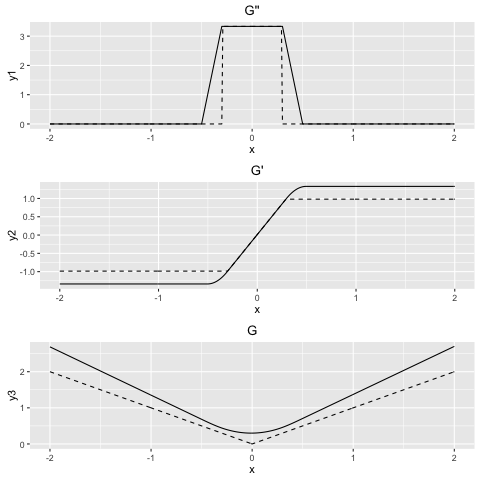
\includegraphics[width=0.35\textwidth]{approximation.png}
\captionof{figure}{Approximation of f}
\end{center}
\end{org}






Let \(n \in \mathbb N^*\) 
Let \(\varepsilon > 0\), \(g \in C^0\) an approximation \(f''_{\varepsilon}\) , such that \(g\) is symmetric and:

\[g_n(x) = \left\{\begin{array}{cc}
0 & \text{if } x \ge \varepsilon + \frac1n \\
\frac1{\varepsilon} \frac{x-\frac1n}{\varepsilon - \frac1n}& \text{when } \varepsilon \le x \le \frac1n + \varepsilon\\
f''_{\varepsilon}(x) & \text{when } x \le \varepsilon
\end{array}\right.
\]
let's call \(G_n(x) = \frac1{\varepsilon} + \int_0^x \int_0^u g_n(s) ds du \in C^2\) 

\(G_n(W_t) = \underbrace{G_n(0)}_{\frac1{\varepsilon}} + \int_0^t G_n'(W_s) dW_s + \int_0^t g_n(W_s) ds\)

It is clear that
\begin{itemize}
\item \(g_n(x) \downarrow f''_{\varepsilon}(x)\)
\item \(|G_n'(x) - f'_{\varepsilon}(x)| \le \frac1n\), so that \(1_{[0, t]} (G_n'(W_t) - f'_{\varepsilon}(W_t))\) converges to \(0\) in \(L_2\).
\item \(G_n(x) \rightarrow f_{\varepsilon}(x)\)
\end{itemize}

We can thus take limits in probability and get:

\(f_{\varepsilon}(W_t) = \frac1{\varepsilon} + \int_0^t f_{\varepsilon}'(W_s) dW_s + \int_0^t f_{\varepsilon}''(W_s) ds\)
\end{document}